\documentclass[fleqn, a4paper, 12pt, twoside]{article}
\usepackage{exsheets} %question and solution environments
\usepackage{amsmath, amssymb, amsthm} %standard AMS packages
\usepackage{esint} %integral signs
\usepackage{marginnote} %marginnotes
\usepackage{gensymb} %miscellaneous symbols
\usepackage{commath} %differential symbols
\usepackage{xcolor} %colours
\usepackage{cancel} %cancelling terms
\usepackage{siunitx} %formatting units
\usepackage{tikz, pgfplots} %diagrams
	\usetikzlibrary{calc, hobby, patterns, intersections, angles, quotes, spy}
\usepackage{graphicx} %inserting graphics
\usepackage{epstopdf} %converting and inserting eps graphics
\usepackage{hyperref} %hyperlinks
\usepackage{datetime} %date and time
\usepackage{ulem} %underline for \emph{}
\usepackage{xfrac, lmodern} %inline fractions
\usepackage{enumerate, enumitem} %numbered lists
\usepackage{float} %inserting floats
\usepackage[american voltages]{circuitikz} %circuit diagrams
\usepackage{pdflscape} %pages in landscape orientation
\usepackage{setspace} %double spacing
\usepackage{microtype} %micro-typography
\usepackage{listings} %formatting code
	\lstset{language=Matlab}
	\lstdefinestyle{standardMatlab}
	{
		belowcaptionskip=1\baselineskip,
		breaklines=true,
		frame=L,
		xleftmargin=\parindent,
		language=C,
		showstringspaces=false,
		basicstyle=\footnotesize\ttfamily,
		keywordstyle=\bfseries\color{green!40!black},
		commentstyle=\itshape\color{purple!40!black},
		identifierstyle=\color{blue},
		stringstyle=\color{orange},
	}
\usepackage{algpseudocode} %algorithms
\usepackage{algorithm} %algorithms

\newcommand\numberthis{\addtocounter{equation}{1}\tag{\theequation}} %adds numbers to specific equations in non-numbered list of equations

\theoremstyle{definition}
\newtheorem{example}{Example}
\newtheorem{definition}{Definition}

\theoremstyle{theorem}
\newtheorem{theorem}{Theorem}
\newtheorem{law}{Law}

\newcommand{\curl}{\mathrm{curl\,}}

\newcommand{\divergence}{\mathrm{div\,}}

\makeatletter
\@addtoreset{section}{part} %resets section numbers in new part
\makeatother

\newcommand\blfootnote[1]{%
	\begingroup
	\renewcommand\thefootnote{}\footnote{#1}%
	\addtocounter{footnote}{-1}%
	\endgroup
}

\renewcommand{\tilde}{\widetilde}

\SetupExSheets{solution/print = true} %prints all solutions by default

%opening
\title{Numerical Analysis}
\author{Aakash Jog}
\date{2015-16}

\begin{document}

\maketitle
%\setlength{\mathindent}{0pt}

\blfootnote
{	
	\begin{figure}[H]
		
\includegraphics[height = 12pt]{cc.eps}
		\includegraphics[height = 12pt]{by.eps}
		\includegraphics[height = 12pt]{nc.eps}
		\includegraphics[height = 12pt]{sa.eps}
	\end{figure}
	This work is licensed under the Creative Commons Attribution-NonCommercial-ShareAlike 4.0 International License. To view a copy of this license, visit \url{http://creativecommons.org/licenses/by-nc-sa/4.0/}.
} %CC-BY-NC-SA license

\tableofcontents

\newpage
\section{Lecturer Information}

\textbf{Naftali Landsberg}\\
~\\
Office: Kitot 215\\
Telephone: \href{tel:+972 3-640-6422}{+972 3-640-6422}\\
E-mail: \href{mailto:naftali.landsberg@gmail.com}{naftali.landsberg@gmail.com}\\
Office Hours: Sundays, 12:00

\section{Recommended Reading}

\begin{enumerate}
	\item B. P. Lathi, Linear Systems and Signals, Oxford University Press (2nd Edition), 2005
	\item Di Stefano et al, Feedback and Control Systems (Schaum’s Outline Series)
	\item D’Azzo, J. and C. Houpis, Linear Control System Analysis \& Design. 4th ed.,
McGraw Hill, 1995
	\item K. Ogata, Modern Control Engineering, Prentice Hall (5th edition 2005)
	\item K. Ogata, Discrete-time control systems, Prentice Hall (2nd Edition 1995)	
\end{enumerate}

\newpage

\section{Classification of Systems}

\begin{enumerate}
	\item Linear and Non-linear
	\item Causal and Non-causal
	\item Time invariant and Time variant
\end{enumerate}

\begin{definition}
	A system is said to be linear if it satisfies the following criteria.
	\begin{enumerate}
		\item Superposition\\
			If $u_1 \to y_1$ and $u_2 \to y_2$, then $\left( u_1 + u_2 \right) \to \left( y_1 + y_3 \right)$.
		\item Homogenity\\
			If $u \to y$, then $\alpha u \to \alpha y$, where $\alpha$ is a constant.
	\end{enumerate}
\end{definition}

\begin{theorem}
	Every linear system can be described by an ODE of the type
	\begin{equation*}
		y^{(n)} + a_{n - 1} y^{(n - 1)} + \dots + a_1 y^{(1)} + a_0 y &= b_m u^{(m)} + \dots + b_1 u^{(1)} + b_0 u
	\end{equation*}
	where $m < n$.
	\label{representation_of_linear_system_by_ODE}
\end{theorem}

\section{Time-domain Analysis of Linear Time-invariant Systems}

\begin{definition}[Step function]
	\begin{align*}
		\delta_{-1}(t) &=
			\begin{cases}
				0 & ;\quad t < 0 \\
				1 & ;\quad t > 0 \\
			\end{cases}
	\end{align*}
\end{definition}

\begin{definition}[Delta function]
	\begin{align*}
		\delta(t) &=
			\begin{cases}
				0          & ;\quad t \neq 0 \\
				\to \infty & ;\quad t = 0    \\
			\end{cases}
	\end{align*}
\end{definition}

\begin{definition}[Ramp function]
	\begin{align*}
		\delta_{-2}(t) &=
			\begin{cases}
				0 & ;\quad t < 0   \\
				t & ;\quad t \ge 0 \\
			\end{cases}
	\end{align*}
\end{definition}

\begin{theorem}
	\begin{align*}
		f(t) \delta(t) & = f(0) \delta(t)
	\end{align*}
\end{theorem}

\begin{theorem}
	\begin{align*}
		\int\limits_{0^-}^{t} f(\tau) \delta(\tau) & = \int\limits_{0^-}^{t} f(0) \delta(\tau) \dif \tau \\
                                                           & = f(0) \quad , \quad t > 0
	\end{align*}
\end{theorem}

\begin{theorem}
	\begin{align*}
		\int\limits_{0^-}^{t} f(\tau) \delta(t - \tau) \dif \tau & = \int\limits_{0^-}^{t} f(t) \delta(t - \tau) \dif \tau \\
                                                                         & = f(t) \int\limits_{0^-}^{t} \delta(t - \tau) \dif \tau \\
                                                                         & = f(t)
	\end{align*}
\end{theorem}

\begin{theorem}
	\begin{align*}
		\int\limits_{0^-}^{t} f(\tau) \delta(t - \tau) \dif \tau & = f(t) \\
                                                                         & = f(t) \ast \delta(t)
	\end{align*}
\end{theorem}

\begin{question}
	Find the solution for
	\begin{align*}
		y^{(2)} + 5 y^{(1)} + 6 y & = u(t) \\
		y(0^-)                    & = 1    \\
		y'(0^-)                   & = 2    \\
		u(t)                      & = \delta_{-1}(t)
	\end{align*}
\end{question}

\begin{solution}
	\begin{align*}
		y^{(2)} + 5 y^{(1)} + 6 y & = u(t)
	\end{align*}
	Therefore, the corresponding homogeneous ODE is
	\begin{align*}
		y^{(2)} + 5 y^{(1)} + 6 y & = 0
	\end{align*}
	Therefore, the corresponding characteristic equation is
	\begin{align*}
		\lambda^2 + 5 \lambda + 6 & = 0
	\end{align*}
	Therefore,
	\begin{align*}
		\lambda_1 & = -2 \\
		\lambda_2 & = -3
	\end{align*}
	Therefore, the ZIR solution is
	\begin{align*}
		y_{\textnormal{ZIR}}(t) & = A e^{\lambda_1 t} + B e^{\lambda_2 t} \\
                                        & = A e^{-2 t} + B e^{-3 t}
	\end{align*}
	Substituting the initial conditions,
	\begin{align*}
		A + B      & = 1 \\
		-2 A - 3 B & = 2
	\end{align*}
	Therefore, the matrix form of the system of equations is
	\begin{align*}
			\begin{pmatrix}
				1  & 1  \\
				-2 & -3 \\
			\end{pmatrix}
			\begin{pmatrix}
				A \\
				B \\
			\end{pmatrix}
		&=
			\begin{pmatrix}
				1 \\
				2 \\
			\end{pmatrix}
	\end{align*}
	Therefore, solving,
	\begin{align*}
		A & = 5 \\
		B & = -4
	\end{align*}
	Therefore,
	\begin{align*}
		y_{\textnormal{ZIR}}(t) & = 5 e^{-2 t} - 4 e_{-3 t}
	\end{align*}
	The ZSR solution is,
	\begin{align*}
		y_{\textnormal{ZSR}}(t) & = \alpha e^{-2 t} + \beta e^{-3 t} + y_p
	\end{align*}
	As $u(t) = \delta_{-1}(t)$,
	\begin{align*}
		y & = c
	\end{align*}
	Therefore, substituting into the ODE, considering zero initial conditions, for $t > 0$,
	\begin{align*}
		6 c & = 1
	\end{align*}
	Therefore,
	\begin{align*}
		y_{\textnormal{ZSR}}(t) & = \left( \alpha e^{-2 t} + \beta e^{-3 t} + \frac{1}{6} \right) \delta_{-1}(t)
	\end{align*}
	As this is a ZSR case, the solution is zero for $t < 0$.
	Hence, $\delta_{-1}(t)$ can be written on the right side.
	This is not necessarily true for the ZIR case.\\
	Therefore,
	\begin{align*}
		y_{\textnormal{ZSR}}(0) & = \frac{1}{6} + \alpha + \beta \\
	\end{align*}
	Also, as the ZSR solution is zero at zero,
	\begin{align*}
		0 & = \frac{1}{6} + \alpha + \beta
	\end{align*}
	Differentiating $y_{\textnormal{ZSR}}(t)$,
	\begin{align*}
		y_{\textnormal{ZSR}}'(0) & = (-2 \alpha - 3 \beta) \delta_{-1}(t) + \left( \frac{1}{6} + \alpha e^{-2 t} + \beta e^{-3 t} \right) \delta(t)
	\end{align*}
	As $f(t) \delta(t) = f(0) \delta(t)$,
	\begin{align*}
		y_{\textnormal{ZSR}}'(0) & = (-2 \alpha - 3 \beta) \delta_{-1}(t) + \left( \frac{1}{6} + \alpha + \beta \right) \delta(t) \\
                                         & = (-2 \alpha - 3 \beta) \delta_{-1}(t)
	\end{align*}
	Therefore, solving,
	\begin{align*}
		\alpha & = -\frac{1}{2} \\
		\beta  & = \frac{1}{3}
	\end{align*}
	Therefore,
	\begin{align*}
		y_{\textnormal{total}}(t) & = y_{\textnormal{ZSR}} + y_{\textnormal{ZIR}}                                                                       \\
                                          & = \left( \frac{1}{6} - \frac{1}{2} e^{-2 t} + \frac{1}{3} e^{-3 t} \right) \delta_{-1}(t) + 5 e^{-2 t} - 4 e^{-3 t} \\
                                          & = \frac{1}{6} + \frac{9}{2} e^{-2 t} - \frac{11}{3} e^{-3 t} \quad , \quad t > 0
	\end{align*}
	~\\
	The same solution can be found by solving for $u(t) = \delta(t)$ and then convolving the solution thus found, and the actual input $u(t) = \delta_{-1}(t)$.\\
	Therefore, the new ODE is
	\begin{align*}
		y^{(2)} + 5 y^{(1)} + 6 y & = \delta(t) \\
		y(0^-)                    & = 0         \\
		y-(0^-)                   & = 0
	\end{align*}
	The impulse response $y_{\delta}$ can be calculated by finding the response for the step function $y_{\delta_{-1}}_{\textnormal{ZSR}}(t)$, and then differentiating it.
	\begin{align*}
		y_{\delta_{-1}}_{\textnormal{ZSR}}(t)       & = \left( \frac{1}{6} - \frac{1}{2} e^{-2 t} + \frac{1}{3} e^{-3 t} \right) \delta_{-1}(t) \\
		\therefore y_{\delta}_{\textnormal{ZSR}}(t) & = \dod{}{t} y_{\delta_{-1}}_{\textnormal{ZSR}}(t)                                         \\
                                                            & = \left( e^{-2 t} - e^{-3 t} \right) \delta_{-1}(t) + \left( \frac{1}{6} - \frac{1}{2} e^{-2 t} + \frac{1}{3} e^{-3 t} \right) \delta(t)
	\end{align*}
	Else, the impulse response $y_{\delta}$ can be calculated by integrating the ODE around zero and finding the new initial conditions for $t = 0^+$.\\
	Therefore,
	\begin{align*}
		y^{(2)} + 5 y^{(1)} + 6 y                                                                                                & = \delta(t) \\
		\therefore \int\limits_{0^-}^{0^+} y'' \dif t + \int\limits_{0^-}^{0^+} 5 y' \dif t + \int\limits_{0^-}^{0^+} 6 y \dif t & = 1
	\end{align*}
	Let
	\begin{align*}
		y''           & = \frac{1}{a} \delta(t)      \\
		\therefore y' & = \frac{1}{a} \delta_{-1}(t) \\
		\therefore y' & = \frac{1}{a} \delta_{-2}(t)
	\end{align*}
	Therefore, substituting,
	\begin{align*}
		y'(0^+) - y'(0^-) + 5 \left( y(0^+) - y(0^-) \right) + 6 \left( \left. \int y \right|_{0^+} - \left. \int y \right|_{0^-} \right) & = 1
	\end{align*}
	Substituting the initial conditions,
	\begin{align*}
		y'(0^+) & = 1
	\end{align*}
	Similarly for $t > 0$.
\end{solution}

\end{document}
